\documentclass[10pt]{beamer}

\usetheme{CambridgeUS}
\usepackage[english, russian]{babel}
\usepackage[utf8]{inputenc}
\usepackage{caption}
\usepackage{minted}
\usepackage{etoolbox}
\usepackage{multicol}
\newcommand{\quotes}[1]{``#1''}
\usepackage{listings}
\usepackage{color}

\definecolor{mygreen}{rgb}{0,0.6,0}
\lstset{
  basicstyle=\ttfamily\footnotesize,        % the size of the fonts that are used for the code
  breaklines=true,                 % automatic line breaking only at whitespace
  captionpos=b,                    % sets the caption-position to bottom
  commentstyle=\color{mygreen},    % comment style
  keywordstyle=\color{blue},       % keyword style
  stringstyle=\color{red},     % string literal style
  showstringspaces=false,
  morekeywords={include, printf},
  texcl=true     %<---- added
}

\title[\href{https://goo.gl/NRgp8K}{https://goo.gl/NRgp8K} (Term 3)]{Виртуальные методы и виртуальное наследование}
\author[Гусев Илья]{Гусев Илья}
\institute[МФТИ] 
{Московский физико-технический институт\\*}
\date{Москва, 2018}
\subject{Computer Science}

\begin{document}

\begin{frame}
  \titlepage
\end{frame}

\begin{frame}{Содержание}
\tableofcontents
\end{frame}

\section{Виртуальные методы}
\subsection{Зачем?}

\begin{frame}[fragile]{Зачем нам виртуальные методы?}
Игрушечный пример:
\begin{lstlisting}[language=C++]
class Animal{
public:
    string do_sound(){ return "WTF"; }
};
class Dog: public Animal{
public:
    string do_sound(){ return "Woof!"; }
};
class Cat: public Animal{
public:
    string do_sound(){ return "Meow!"; }
};
\end{lstlisting}
Хочется собрать всех животных и заставить их издавать звуки, присущие конкретному животному. Но мы не можем положить разнородные объекты в массив. Давайте положим их указатели на Animal!
\end{frame}

\begin{frame}[fragile]{Зачем нам виртуальные методы?}
\begin{lstlisting}[language=C++]
#include <vector>
using namespace std;

int main(){
    B dog;
    C cat;
    vector<A*> animals;
    animals.push_back(&B);
    animals.push_back(&C);
    for( A* ptr: animals ) {
        cout<<ptr->do_sound()<<" ";
    }
}
\end{lstlisting}
Вывод: "WTF WTF".

А как нам например, обрабатывать коллекцию окон в ОС? Использовать сложные иерархии? 
\end{frame}

\begin{frame}[fragile]{Зачем нам виртуальные методы?}
\begin{lstlisting}[language=C++]
class Animal{
public:
    virtual string do_sound(){ return "WTF"; }
};
class Dog: public Animal{
public:
    string do_sound(){ return "Woof!"; }
};
class Cat: public Animal{
public:
    string do_sound(){ return "Meow!"; }
};
\end{lstlisting}
Тот же main.

Вывод: "Woof! Meow!".
\end{frame}

\begin{frame}[fragile]{Зачем нам виртуальные методы?[2]}
Старый код вызывает новый код.
\begin{lstlisting}[language=C++]
class Animal{
public:
    string say() { return do_sound()+do_sound(); }
    virtual string do_sound(){ return "WTF"; }
};
class Dog: public Animal{
public:
    string do_sound(){ return "Woof!"; }
};
class Cat: public Animal{
public:
    string do_sound(){ return "Meow!"; }
};

\end{lstlisting}
\end{frame}

\subsection{Использование}
\begin{frame}[fragile]{Виртуальные методы}
\begin{enumerate}
    \item Синтаксис - ключевое слово virtual перед методом базового класса.
    \item virtual у методов производных классов опционален, но лучше писать для понятности.
    \item Чисто виртуальные функции: virtual void foo() = 0;
    \item Если функция виртуальная, то какая именно функция определяется в runtime, а не на этапе компиляции.
    \item Если у класса есть хотя бы одна виртуальная функция, деструктор тоже следует сделать виртуальным. Почему?
    \item Преобразования по иерархии через dynamic\_cast (для безопасности).
\end{enumerate}
\end{frame}


\begin{frame}[fragile]{Виртуальный деструктор}
\begin{lstlisting}[language=C++]
class Base {
public:
    ~Base();
};

class Derived : public Base {
public:
    ~Derived();
};

void f()
{
    Base* p = new Derived;
    delete p;  // деструктор Derived не вызывается
}
\end{lstlisting}
А если в деструкторе происходило освобождение ресурсов (закрытие файлового десриптора, особождение по указателям полей)?
\end{frame}


\subsection{Как это работает?}
\begin{frame}[fragile]{Как это работает}
\begin{enumerate}
    \item Полностью определяется компилятором!
    \item Всегда есть v-table.
    \item Рассмотрим на примере
\end{enumerate}
\end{frame}

\begin{frame}[fragile]{Как это работает}
Такой класс:
\begin{lstlisting}[language=C++]
class Base {
public:
  virtual int virt0();
  virtual int virt1();
  virtual int virt2();
  virtual int virt3();
};
\end{lstlisting}
\end{frame}


\begin{frame}[fragile]{Как это работает}
Шаг 1: компилятор создаёт статическую таблицу с указателями на функции.
\begin{lstlisting}[language=C++]
// Псевдокод для статической таблицы в Base.cpp
// Притворимся, что FunctionPtr - это указатель на метод
FunctionPtr Base::__vtable[4] = {
  &Base::virt0, &Base::virt1, &Base::virt2, &Base::virt3
};
\end{lstlisting}
\vspace{5mm}
Шаг 2: компилятор добавляет скрытый указатель (обычно void*) к каждому объекту класса Base. Этот указатель обычно называют v-pointer. Можно представлять, что компилятор переписывает класс примерно так:

\begin{lstlisting}[language=C++]
class Base {
public:
  // ...
  FunctionPtr* __vptr;  // подставляется компилятором, скрыт
  // ...
};
\end{lstlisting}
\end{frame}

\begin{frame}[fragile]{Как это работает}
Шаг 3: компилятор инициализирует this->\_\_vptr в каждом конструкторе. Можно представлять, что в списко ицнициализации добаляется привязка к v-table:
\begin{lstlisting}[language=C++]
Base::Base()
  : __vptr(&Base::__vtable[0])  // подставляется компилятором
  // ...
{
  // ...
}
\end{lstlisting}
\end{frame}

\begin{frame}[fragile]{Как это работает}
Для производного класса выполняются шаги 1 и 3 (но не 2). Предположим, что Derived переопределяет virt0 и virt1. Тогда:
\begin{lstlisting}[language=C++]
FunctionPtr Der::__vtable[5] = {
  &Der::virt0, &Der::virt1, &Base::virt2, &Base::virt3
};
\end{lstlisting}
В итоге этот код:
\begin{lstlisting}[language=C++]
void mycode(Base* p)
{
  p->virt3();
}
\end{lstlisting}
Трансофрмируется в этот (псевдокод):
\begin{lstlisting}[language=C++]
void mycode(Base* p)
{
  p->__vptr[3](p);
}
\end{lstlisting}
\end{frame}

\begin{frame}[fragile]{Пример реального расположения для g++}
\begin{lstlisting}[language=C++]
class A{
public:
    virtual void doSomeWork();
};

class B : public A{
public:
    virtual void doSomeWork();
};
\end{lstlisting}
\end{frame}

\begin{frame}[fragile]{Пример реального расположения для g++}
Команда: g++ -fdump-class-hierarchy example.h
\begin{multicols}{2}
\begin{lstlisting}[language=C++]
Vtable for A
A::_ZTV1A: 3u entries
0     (int (*)(...))0
8     (int (*)(...))(& _ZTI1A)
16    (int (*)(...))A::doSomeWork

Class A
   size=8 align=8
   base size=8 base align=8
A (0x7fb76785a4) 0
    vptr=((& A::_ZTV1A) + 16u)
\end{lstlisting}
\vfill\eject
\begin{lstlisting}[language=C++]
Vtable for B
B::_ZTV1B: 3u entries
0     (int (*)(...))0
8     (int (*)(...))(& _ZTI1B)
16    (int (*)(...))B::doSomeWork

Class B
   size=8 align=8
   base size=8 base align=8
B (0x7fb7678510) 0
    vptr=((& B::_ZTV1B) + 16u)
  A (0x7fb76785a540) 0
      primary-for B (0x7fb7678510)
\end{lstlisting}
\end{multicols}
\end{frame}

\section{Вирутальное наследование}
\subsection{Зачем?}

\begin{frame}[fragile]{Обычное наследование - контрольные вопросы}
\begin{enumerate}
\item Чем struct отличается от class по стандарту?
\item А по смыслу?
\item Зачем нужно наследование?
\item Типы наследования.
\item Зачем нужно приватное наследование, примеры использвоания
\item Композиция vs наследование
\item friend - что это?
\item Концепция интерфейсов.
\item ABC
\end{enumerate}
\end{frame}

\begin{frame}[fragile]{Обычное наследование}
B наследуется от A
\begin{lstlisting}[language=C++]

struct A {
    int a;
    
    void foo(){}
};

struct B: A {
    int b;
    
    void foo(){}
};

sizeof(int) == 4;
sizeof(A) == ?;
sizeof(B) == ?;

B objectB;
\end{lstlisting}
Как вызвать foo() из A?
\end{frame}

\begin{frame}[fragile]{Множественное наследование}
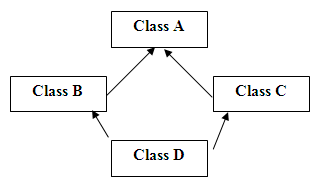
\includegraphics[width=8cm, height=5cm]{Term_3/Source/Pictures/virtual-inheritance.png}
\end{frame}

\begin{frame}[fragile]{Множественное наследование}
\begin{lstlisting}[language=C++]
struct A {
    int a = 4;
    void foo(){}
};

struct B: public A {
    int b = 5;
    void foo(){}
};

struct C: public A {
    int c = 6;
    void foo() {}
};

struct D: public B, public C {
    int d = 7;
    void foo() {}
};
\end{lstlisting}
\end{frame}

\begin{frame}[fragile]{Множественное наследование}
\begin{lstlisting}[language=C++]
sizeof(D) == ?

int GetShiftedInt(int& a, int n) {
    return *((int*)(&a) - n);
}

int main(){
    D objectD;
    int& d = objectD.d;
    cout<<d<<" "<<GetShiftedInt(d, 1)<<" "<<GetShiftedInt(d, 2)<<
    " "<<GetShiftedInt(d, 3)<<" "<<GetShiftedInt(d, 4)<<endl;
}


\end{lstlisting}
\end{frame}

\begin{frame}[fragile]{Множественное виртуальное наследование}
\begin{lstlisting}[language=C++]
struct A {
    int a = 4;
    void foo(){}
};

struct B: public virtual A {
    int b = 5;
    void foo(){}
};

struct C: public virtual A {
    int c = 6;
    void foo() {}
};

struct D: public B, public C {
    int d = 7;
    void foo() {}
};
\end{lstlisting}
\end{frame}

\begin{frame}[fragile]{Множественное виртуальное наследование}
\begin{lstlisting}[language=C++]
sizeof(D) == ?

\end{lstlisting}
\end{frame}


\begin{frame}[fragile]{Виртуальное наследование - особенности}
\begin{enumerate}
\item Ни в коем случае не использовать C-style cast, вместо этого - dynamic\_cast
\item Внимательнее с порядком вызова конструкторов. В целом - сверху вниз, слева направо в графе наследования.

\end{enumerate}
\end{frame}


\appendix
\section<presentation>*{\appendixname}
\subsection<presentation>*{Useful links}

\begin{frame}[allowframebreaks]
  \frametitle<presentation>{Полезные ссылки}
    
  \begin{thebibliography}{10}
{
  \beamertemplatebookbibitems
  % Start with overview books.
    
\bibitem{faq}
  \texttt{C++ Super-FAQ}
  \newblock \href{https://isocpp.org/wiki/faq/virtual-functions}{\texttt{https://isocpp.org/wiki/faq/virtual-functions}}
  
 \bibitem{so1}
  \texttt{SO - Virtual Table layout in memory?}
  \newblock \href{https://stackoverflow.com/questions/1342126/virtual-table-layout-in-memory}{\texttt{https://stackoverflow.com/questions/1342126/virtual-table-layout-in-memory}}
}

\bibitem{object model}
  \texttt{g++ object model}
  \newblock \href{http://spockwangs.github.io/2011/01/31/cpp-object-model.html}{\texttt{http://spockwangs.github.io/2011/01/31/cpp-object-model.html}}
  
 \bibitem{object model}
  \texttt{Цикл статей по устройству vtable в clang}
  \newblock \href{https://shaharmike.com/cpp/vtable-part1/}{\texttt{https://shaharmike.com/cpp/vtable-part1/}}
  


    
  \end{thebibliography}
\end{frame}

\end{document}


